\documentclass{standalone}

\usepackage{tikz}
\usetikzlibrary{arrows}
\usetikzlibrary{arrows.meta}
\usetikzlibrary{positioning}
\usetikzlibrary{math}

% For correctly centering Dbar
\newlength{\dwidth}
\newlength{\shift}

\begin{document}
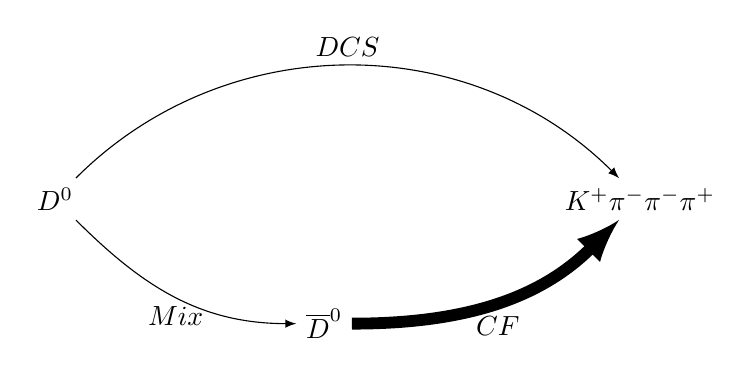
\begin{tikzpicture}
    \node (D) {$D^0$};

    % Try and make the D bar aligned
    \settowidth{\dwidth}{\pgfinterruptpicture $\overline{D}^0$ \endpgfinterruptpicture}
    \tikzmath{
    \shift=\dwidth/-2;}
    
    \node (Dbar) [below right=1cm and \shift+3cm of D] {$\overline{D}^0$};
    \node (f) [right=6cm of D] {$K^+\pi^- \pi^- \pi^+$};

    \draw[-{latex[scale=10.0]}] (D) edge[out=45, in=135] node[above] {$DCS$} (f);

    \draw[-{latex[scale=10.0]}] (D) edge[out=-45, in=180] node[below]{$Mix$} (Dbar);
    \draw[-latex, line width=1.5mm] (Dbar) edge[out=0, in=-135] node[below]{$CF$} (f);
\end{tikzpicture}
\end{document}

